\chapter{Results and Discussion}
\label{ch:results}

\section{Compliance with the registered proposal}

\begin{table}[H]
\centering
\caption{Registered milestones compared with the implemented project.}
\label{tab:proposal-compliance}
\begin{tabularx}{\textwidth}{@{}p{0.25\textwidth}p{0.27\textwidth}X@{}}
\toprule
Proposal item & Status & Implemented outcome\\
\midrule
PyTorch--NGSolve bridge
& Achieved
& Integration-point transfer, custom Newton loop, and exact AD derivatives
were implemented and verified.\\
Periodic particle RVE
& Achieved and extended
& Native periodic spaces were combined with a mixed matrix and exact rigid
particle surface kinematics.\\
Rigid glass penalty
& Replaced
& The proposed \(E\rightarrow\infty\) penalty was rejected in favor of exact
finite rigid motion and free moment equilibrium.\\
Numerically perturbed RVE tangent
& Replaced
& The tangent is obtained from symbolic differentiation and Schur
condensation; perturbations are used only for verification.\\
\(6\times6\) Voigt mapping
& Corrected
& The total-Lagrange derivative \(\partial\Pstress/\partial\F\) is retained as
the full row-major \(9\times9\) tangent.\\
Parameterized pICNN and dataset
& Achieved
& Deterministic schema-2 datasets, grouped splits, training/fine-tuning, and
constitutive checks were completed and frozen with hashes.\\
Macroscopic demonstration
& Achieved for first-order integration; partly achieved overall
& First-order runs reached 5\%; the selected shear fine-tune
also completed a matched macro-FE run. Second-order mesh refinement is
available at 0.5\%, but a second-order 5\% run and
quadrature convergence remain incomplete.\\
\bottomrule
\end{tabularx}
\end{table}

\section{Phase 1 constitutive bridge}

The committee-requested proof of concept was completed before the RVE
production campaigns began: the Phase~1 pICNN passed the reference-state,
analytical-response, tangent, nonlinear-equilibrium, affine-patch, and
matched finite-element checks. The matched
analytical-versus-neural FE benchmark gave relative errors of
1.376\% in free displacement,
0.3504\% in deformation gradient, and
13.60\% in reaction vector. The reaction error is acceptable
for the proof-of-concept gate but is not evidence of a production constitutive
surrogate.

\section{RVE equilibrium and homogenization}

\begin{table}[H]
\centering
\caption{Selected verified Phase~2 results.}
\label{tab:p2-results}
\begin{tabular}{@{}lr@{}}
\toprule
Quantity & Result\\
\midrule
Maximum periodic displacement jump & \(1.466\times10^{-20}\)\\
Rigid-particle trace error & \(8.269\times10^{-19}\)\\
Final free-rotation moment residual & \(1.436\times10^{-15}\)\\
Hill--Mandel relative power error & \(1.085\times10^{-13}\)\\
Condensed-tangent major-symmetry error & \(5.169\times10^{-16}\)\\
Tangent Taylor remainder orders & \(2.000,\ 2.000\)\\
Translation-gauge homogenized-stress change & \(6.827\times10^{-13}\)\\
\bottomrule
\end{tabular}
\end{table}

Under simple shear, free rotation converged in three outer Newton iterations
from a moment residual of \(4.751\times10^{-3}\) to
\(1.436\times10^{-15}\). The particle rotation remained proper orthogonal,
and the condensed rotational Hessian was symmetric to
\(1.732\times10^{-17}\).

\section{Dataset and surrogate}

The pilot dataset contains 300 samples. Stored integrity checks confirmed
complete sample IDs, split consistency, reference states, proper rotations,
and finite arrays. The maximum recorded residuals were
\(8.632\times10^{-11}\) for mixed equilibrium,
\(9.948\times10^{-10}\) for rotational equilibrium, and
\(9.563\times10^{-13}\) for condensation. The maximum tangent-symmetry error
was \(1.144\times10^{-15}\).

\begin{figure}[htbp]
\centering
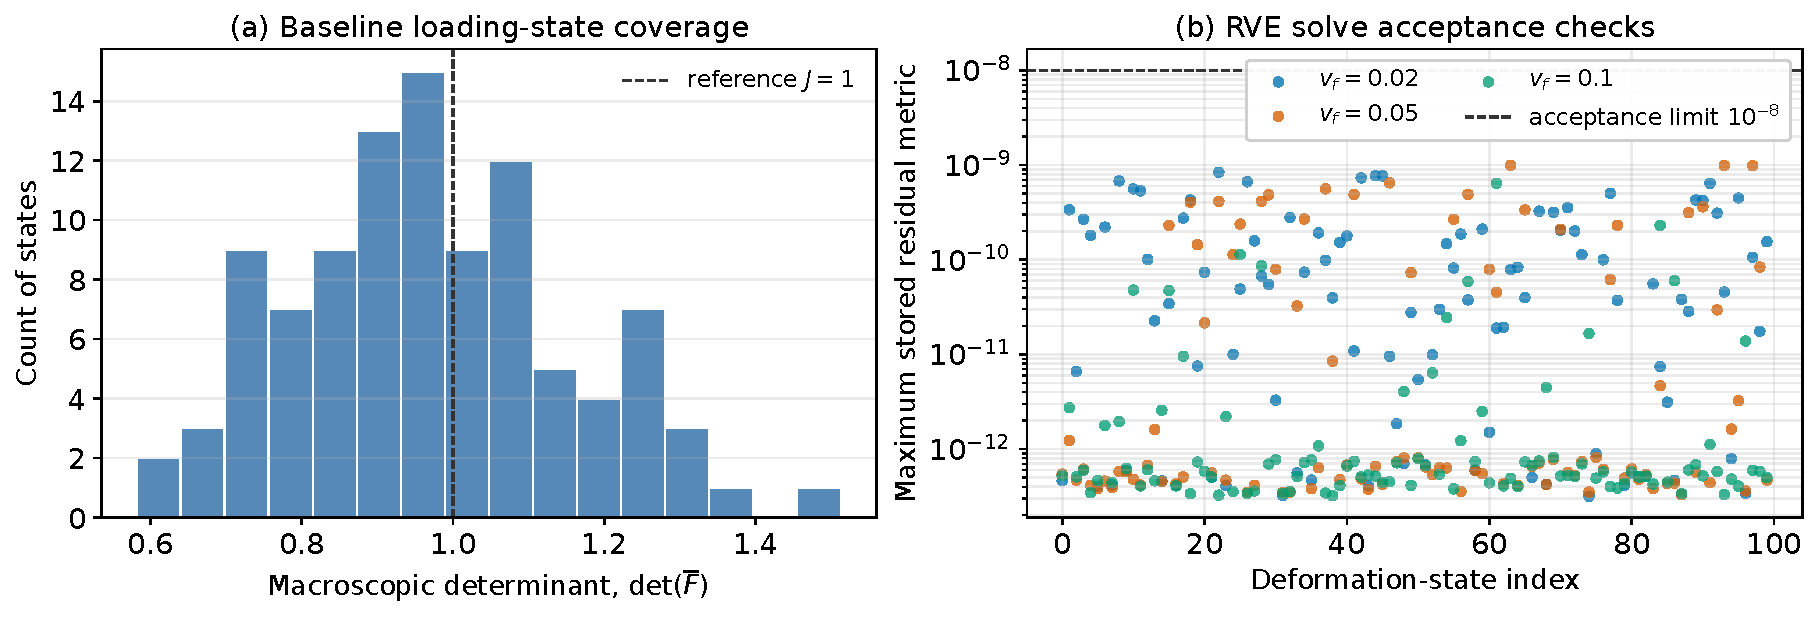
\includegraphics[width=\textwidth]{phase2_pilot_coverage_and_residuals}
\caption{Integrity diagnostics for the 300-record Phase~2 pilot dataset.
(a) Distribution of \(\det\Fbar\) over its 100 unique macroscopic loading
states, counted once rather than repeated for each volume fraction.
(b) Maximum stored residual metric per record, defined as the largest of
the mixed-equilibrium norm, particle-moment residual, and condensed
sensitivity residual. These residual channels have different meanings, but
each was required to remain below \(10^{-8}\). This pilot-coverage plot is
not the targeted Phase~6 training-set distribution.}
\label{fig:phase2-pilot-diagnostics}
\end{figure}

This limitation was corrected in schema version~2. The later 300-, 900-,
1080-, 1260-, and 600-record datasets store per-sample minimum and maximum
microscopic Jacobians, solver status, iteration counts, and residuals. For
example, the Phase~6 training dataset contains 1260 records at
\(\vfrac=0.02,0.05,0.10\), with targeted compression
\(J\in[0.51,0.60]\), expansion \(J\in[1.50,1.80]\), and dataset SHA-256
\texttt{9e8a47be77ce7fb5076d73744c50f753374fc0741b6a64cc0dcff2990fdc1b26}.

The Phase~6 checkpoint was evaluated on a newly generated Phase~7 dataset
with a different seed and 531 eligible held-out records. Overall energy RMSE
was 1.373 (normalized by the training RMS: \(1.402\times10^{-3}\)); stress
component RMSE was 5.740 (normalized: \(2.352\times10^{-3}\)). The tangent
relative Frobenius error had mean \(8.467\times10^{-3}\), median
\(4.916\times10^{-3}\), 90th percentile \(1.901\times10^{-2}\), and maximum
\(6.012\times10^{-2}\). Worst energy and stress errors both occurred at
\texttt{v002\_f000180}; the worst tangent record was
\texttt{v002\_f000023}. This independent evaluation belongs to checkpoint
\texttt{2efa831c...196d}, not to the later fine-tuned model.

The Phase~6/7 base fine-tuned checkpoint \texttt{32b0a41f...fea70} selected epoch 2750.
Validation energy and stress RMSEs were 0.344 and 1.771, and validation tangent
relative Frobenius RMSE was \(2.688\times10^{-3}\). Its grouped holdout energy
and stress RMSEs were 0.519 and 2.466. Because the Phase~7 source set had
previously been used for evaluation of the earlier model, these final-model
figures are reported as held-out numerical metrics, not as a fresh independent
generalization result.

\subsection{Shear adaptation and independent evaluation}

The selected full shear fine-tune (checkpoint SHA-256 prefix
\texttt{5c1c606057eb}) was evaluated against the frozen Phase~6/7 checkpoint
(prefix \texttt{32b0a41fdd75}); the full digests are listed in
Appendix~\ref{app:reproducibility}. The 12 scored direct-RVE cases span four
positive simple-shear amplitudes (\(\gamma=0.015\), \(0.0325\), \(0.0725\),
and \(0.0975\)) at all three volume fractions. Three identity records were
included for auditing and excluded from error metrics.
The final set used microstructure seed 20261116, distinct from the adaptation
seed, and was generated after model selection.

\begin{table}[H]
\centering
\caption{Independent simple-shear errors for the frozen Phase~6/7 checkpoint
and selected full shear fine-tune. Errors are percentages; each
volume-fraction row contains four cases.}
\label{tab:final-shear-vf}
\begin{tabular}{@{}lrrrrrr@{}}
\toprule
Volume fraction & \multicolumn{2}{c}{\shortstack{Mean relative P\(_{01}\)\\error (\%)}} &
\multicolumn{2}{c}{\shortstack{Mean relative tangent\\error (\%)}} &
\multicolumn{2}{c}{\shortstack{Stress Frobenius\\relative RMSE (\%)}}\\
& Frozen & Fine-tuned & Frozen & Fine-tuned & Frozen & Fine-tuned\\
\midrule
0.02 & 45.9 & 28.9 & 45.8 & 28.9 & 50.3 & 34.5\\
0.05 & 55.3 & 37.0 & 55.3 & 37.0 & 59.8 & 42.5\\
0.10 & 75.3 & 54.4 & 75.1 & 54.2 & 79.5 & 59.4\\
\bottomrule
\end{tabular}
\end{table}

\begin{table}[H]
\centering
\caption{Independent simple-shear errors grouped by amplitude. Each row
contains the three volume fractions.}
\label{tab:final-shear-amplitude}
\begin{tabular}{@{}lrrrrrr@{}}
\toprule
Shear amplitude & \multicolumn{2}{c}{\shortstack{Mean relative P\(_{01}\)\\error (\%)}} &
\multicolumn{2}{c}{\shortstack{Mean relative tangent\\error (\%)}} &
\multicolumn{2}{c}{\shortstack{Stress Frobenius\\relative RMSE (\%)}}\\
& Frozen & Fine-tuned & Frozen & Fine-tuned & Frozen & Fine-tuned\\
\midrule
0.0150 & 58.8 & 40.1 & 58.8 & 40.1 & 60.4 & 41.8\\
0.0325 & 58.8 & 40.1 & 58.8 & 40.1 & 61.3 & 42.9\\
0.0725 & 58.8 & 40.1 & 58.7 & 40.0 & 65.6 & 48.1\\
0.0975 & 58.7 & 40.1 & 58.6 & 39.9 & 69.7 & 52.8\\
\bottomrule
\end{tabular}
\end{table}

Overall mean relative energy error fell from 58.82\% to 40.12\%, mean relative
P\(_{01}\) error from 58.80\% to 40.11\%, and mean relative tangent error
from 58.73\% to 40.04\%. Stress Frobenius relative RMSE fell from 64.33\% to
46.62\%. The candidate improved in every volume-fraction and amplitude group.
Its relative stress error increased with amplitude, from 41.8\% at
\(\gamma=0.015\) to 52.8\% at \(\gamma=0.0975\). The small group sizes
(three cases per amplitude and four
per volume fraction) and the single new microstructure seed limit the scope
of this result. Remaining errors are substantial; the fine-tune improves
shear response but does not remove its bias.

\section{Macroscopic finite-element status}

Early residual-merit trials stalled near 2--3.2\% stretch. Replacing residual
merit by the energy merit function and adding a secant load predictor allowed
the first-order Phase~6/7 reference model to complete 100 load steps to
5\% stretch at three meshes:
\begin{center}
\begin{tabular}{@{}rrrrr@{}}
\toprule
\(h\) & Elements & DOFs & Final residual & Minimum sampled \(J\)\\
\midrule
0.25 & 399 & 405 & \(1.629\times10^{-10}\) & 0.9694\\
0.20 & 648 & 642 & \(3.790\times10^{-12}\) & 0.9686\\
0.16 & 1818 & 1356 & \(1.044\times10^{-12}\) & 0.9801\\
\bottomrule
\end{tabular}
\end{center}
All three reports mark the sampled states finite and orientation-preserving.
This proves solver completion, not mesh convergence of a response quantity.
Moreover, the second-order \(h=0.20\) trial failed near 0.82\% stretch and the
second-order \(h=0.25\) trial failed near 0.28\%.

At the smaller target stretch of 0.5\%, a second-order,
quadrature-order-4 mesh refinement completed at \(h=0.25,0.20,0.16\):
\begin{center}
\begin{tabular}{@{}rrrr@{}}
\toprule
\(h\) & Final energy & Final free residual & Minimum sampled \(J\)\\
\midrule
0.25 & \(8.542666041\times10^{-5}\) & \(2.947\times10^{-9}\) & 0.999938\\
0.20 & \(8.356703682\times10^{-5}\) & \(3.348\times10^{-11}\) & 0.999936\\
0.16 & \(8.291093705\times10^{-5}\) & \(2.663\times10^{-13}\) & 0.999853\\
\bottomrule
\end{tabular}
\end{center}
The relative energy changes were 2.23\% from \(h=0.25\) to \(0.20\), 0.79\%
from \(0.20\) to \(0.16\), and 3.03\% from \(0.25\) to \(0.16\). This is
small-load mesh-refinement evidence only; it does not establish second-order
convergence at the 5\% target.

The selected shear fine-tune completed a matched macro-FE run with the same
first-order setup as the frozen reference (\(\vfrac=0.05\), \(h=0.25\),
quadrature order 4, energy merit, secant predictor, and 100 load steps):
\begin{center}
\begin{tabular}{@{}lrrrr@{}}
\toprule
Checkpoint & Final stretch & Final residual & Minimum sampled \(J\) & Final energy\\
\midrule
Frozen Phase~6/7 & 0.05 & \(1.6295\times10^{-10}\) & 0.969439 & 0.7158683421\\
Selected shear fine-tune & 0.05 & \(1.0743\times10^{-12}\) & 0.969393 & 0.7205473194\\
\bottomrule
\end{tabular}
\end{center}
The relative final-energy difference was 0.649\%. Both runs completed with
positive sampled Jacobians. This confirms macro-FE integration for the
selected checkpoint at this matched mesh; it does not show mesh-independent
energy convergence. The remaining limitations are:
\begin{enumerate}
  \item complete second-order macro-FE paths to the 5\% target;
  \item establish broader mesh and quadrature convergence;
  \item test more microstructure realizations and loading paths; and
  \item compare against physical PDMS--glass data.
\end{enumerate}
No final claim of mesh-independent component response is made at this stage.
